%!TEX root = ../dissertation.tex
\chapter{Software Implementation Aspects}
\label{chap:implementation}
This chapter provides details about the software implementation of the multi-physics simulation framework discussed in this thesis along with specifics about the parallel computing approach.  The software implementation is an open-source platform called Chrono, and is released in public domains under a BSD3 license \cite{projectChronoGithub,chronoOverview2016}. Chrono is a cross-platform (Windows/Linunx/MacOS) middleware and can be embedded in third-party applications. It is modular and expandable via C++ inheritance and run-time polymorphism.

The high-level overview of the simulation algorithm is as follows. Each subsystem is responsible for advancing its state to the next simulation time-step. Subsequently, solutions are coupled at the interface of the continuum and discrete subsystems as shown in Fig.~\ref{fig:fsi_FD}. This strategy allows each subsystem to work independently of others within a time-step, and to choose a suitable parallelization paradigm. 

\section{Overview of Chrono}
Chrono is a physics-based parallel-computing modeling and simulation infrastructure based on a platform-independent and open-source design in C++.  Chrono can be employed for solving a wide range of mechanical systems featuring rigid and flexible body dynamics, fluid dynamics, and in fluid-solid interaction problems. 
The core Chrono engine allows for simulation of mechanisms made of rigid bodies and constraints using a wide set of joints. It allows for applying motors, linear actuators, springs and dampers as well as forces and torques. The finite element functionality allows for modeling flexible parts with beams, cables, shells, solid tetrahedrons and hexahedrons elements and for non-linear analysis with large deformations. Chrono allows for modeling more involved mechanical systems such as vehicles using a template-based approach, leveraging a wide set of suspension templates as well as soil and tire models and powertrains/drivelines.
The fluid dynamics module allows for CFD simulations, and is discussed in the rest of this thesis. The schematic overview of Chrono is illustrated in Fig.~\ref{fig:chrono}.
\begin{figure}[H]
	\begin{center}
		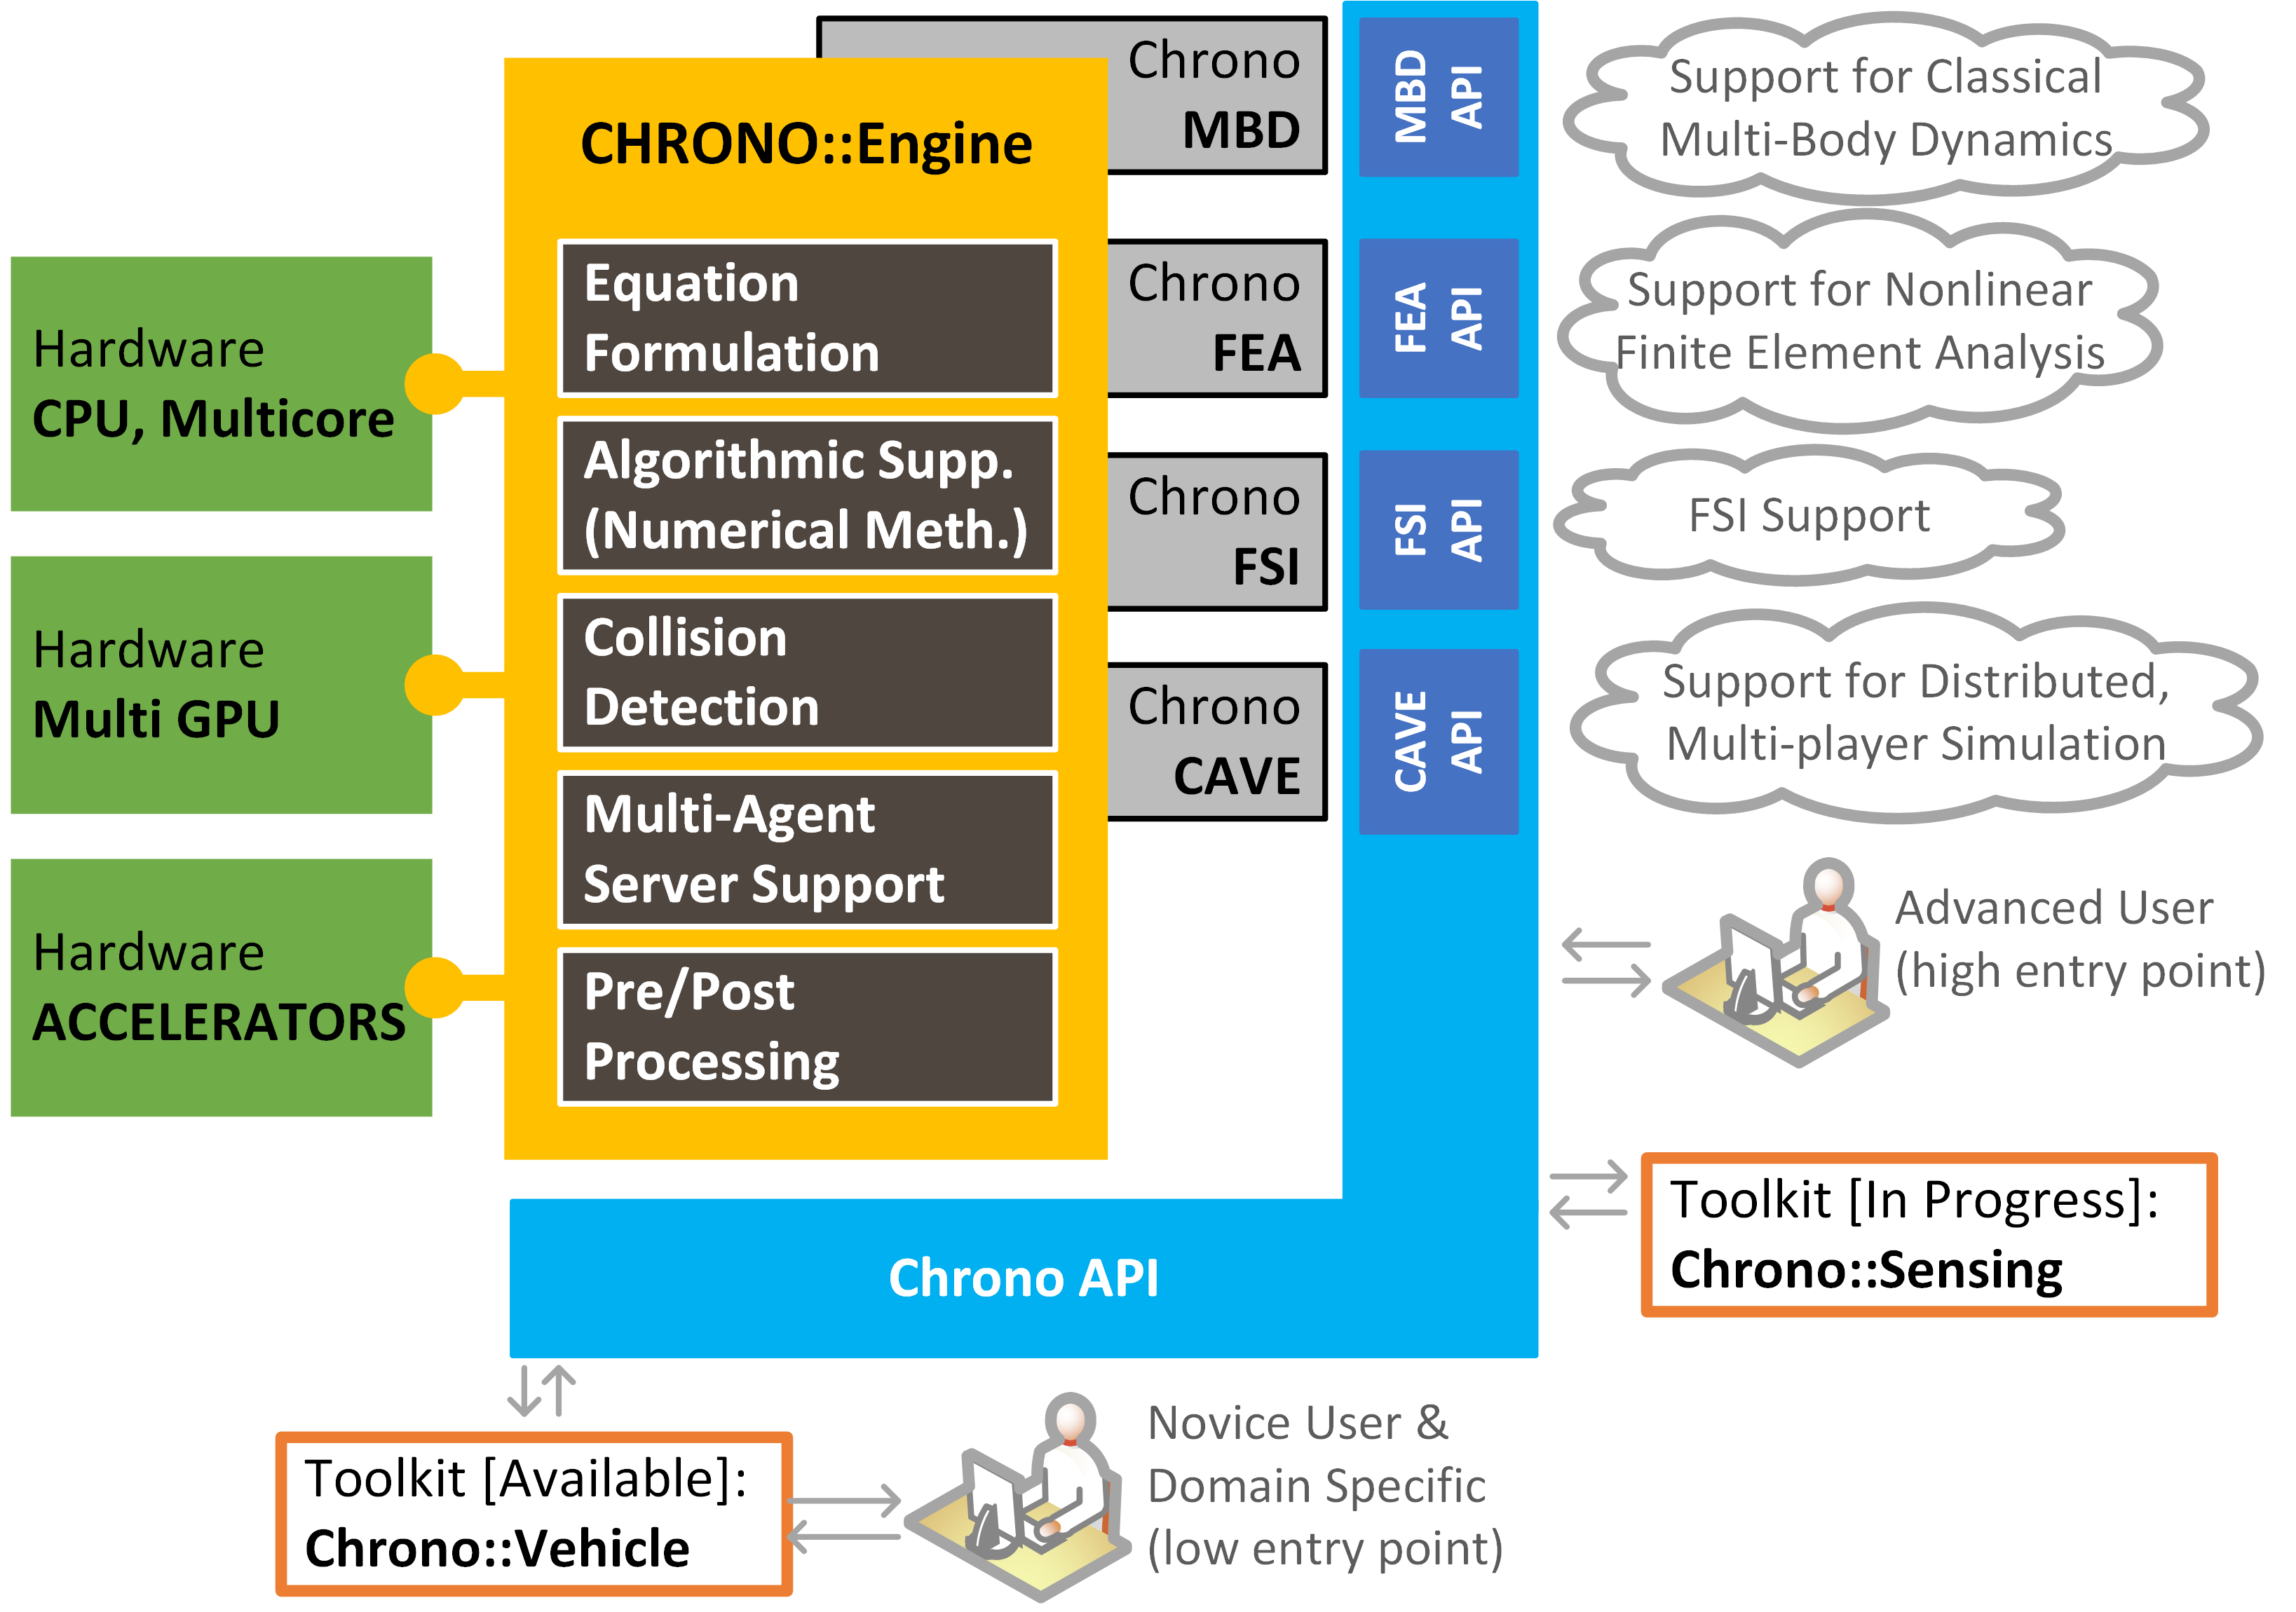
\includegraphics[width=.9\linewidth]{images/chronoStructure.png}
	\end{center}
	\caption{Structure of Chrono and its submodules.}
	\label{fig:chrono}
\end{figure}


\section{Parallel Computing}
The purpose of the rest of this chapter is to elaborate the use of parallel computing to accelerate computational multi-physics platform discuss in the present thesis.  Parallel computing is becoming increasingly important in multi-physics simulation. This is the case because most  real-world problems involve a large number of degrees of freedom, which cannot be efficiently handled via only a single core. The following keypoints summarize the main reasons behind this shift from sequential to parallel computing. 
\begin{itemize}
	\item The growing disparity between memory access speed and CPU processing speed, the memory wall, still poses a challenge.  This is the case because CPU speeds have increased regularly, while memory speed, in terms of both the bandwidth and the latency, has increased at a significantly lower rate. 
	\item Instruction-level parallelism achieved through branch prediction, out-of-order execution and speculation would require longer horizons and higher power consumption to gain further improvements.
	\item Increasing the CPU clock-cycle leads to exponentially-growing energy sinks, which would require significant improvement in the cooling strategies.
\end{itemize}
Hence, exploiting parallel computing is necessary to ensure that computer simulation remains a viable alternative to experimental methods. Herein, the discrete system component of the solution is the legacy solution implemented in Chrono augmented to support two-way FSI coupling via BCE markers. It runs on the CPU leveraging multi-core parallelism. The continuum component of the solution was implemented on the GPU, an architecture suitable for fine-grained parallelism of the single-instruction-multiple-data type calculation encountered in SPH discretization. Leveraging hybrid parallel computing by using a multi-core CPU solution for the discrete phase and a GPU solution for the continuum phase allows to fully exploit all computational hardware assets available on modern workstations.


\subsection{CPU Computing Approach}
Amongst parallel programming models, the distributed-memory multi-processor architecture, and shared-memory multi-processor architecture are prime examples that have proven effective for high-level parallelization. 

%In the distributed-memory multi-processor paradigm, each process has its own address space, but communication among processes can be done through fast interconnection network such as Mellanox and InfiniBand via APIs such as Message Passing Interface (MPI).  MPICH and OpenMPI are various implementations of MPI standards. 

In the shared-memory multi-processor paradigm, all the processes share the same address space, i.e., each processor has direct access to the same memory.  This model can be leveraged by  APIs such as OpenMP, which offers a low overhead and high-level means to achieve parallelism. In the OpenMP model, compilers generate parallel execution regions through the use of directives. This idea allows for generating portable and reasonably scalable code, and running on a wide variety of machines. Most notably, these directives will be safely ignored on a machine without an OpneMP library and the code will be run sequentially.

In the present work, OpenMP is used for parallelization of computationally intensive parts of the flexible body dynamics solver. More specifically, computation of the internal loads (see Eqs.~\ref{eq:ANCF_Beam_Qe} and \ref{eq:equ11}) and the system Jacobian elements  are parallelized via OpenMP \textit{parallel for} constructs.

Lastly, Advanced Vector Extension (AVX) intrinsics are used for parallelizing low-level math operations in this work. The idea of AVX, and other math vectorizing extensions such as SSE, is to perform a single instruction on multiple pieces of data. This is relevant when working with low-level matrix operations. For instance, four floats (or two doubles) can be packed into a single 128 bit register, and one instruction can add the four floats. This idea makes the underlying matrix operations faster and improves the efficiency of the simulations. 

\subsection{GPU Computing Approach}
GPU computing model is based on the concept of a compute accelerator. In this model, a device separate from the host performs computational tasks and transfer data back to the host once needed. Graphics Processing Unit (GPU) and Intel's Xeon Phi are prime examples of such models. 

The hardware of GPUs is different from their CPU counterparts in many ways. One key architectural difference between CPU and GPU is in the number of physical cores; while a CPU has fewer of more powerful cores, a GPU has more of less powerful physical cores. GPU physical cores also run at a lower clock speed. Given this special architecture, GPUs had been originally designed for video gaming and displaying complex graphics, where rendering processing hundreds of thousands of polygons in each frame is necessary. Therefore, ``single instruction multiple data'' (SIMD) is the parallel paradigm that describes the programming model suitable for GPU computing.

NVIDIA facilitated the use of such devices for computing purposes through the Compute Unified Device Architecture (CUDA) API and libraries, which assist with building blocks in computational science. In the present work, the pressure equation is solved via Krylov subspace methods \cite{saad2003iterative,vdVorst2003}. For matrix-vector and vector dot product operations, our Krylov-subspace linear solver relies on two linear algebra libraries provided by NVIDIA: cuSPARSE \cite{cuSparse2014} and cuBLAS \cite{cuBlas}. 

